\section{Dataset}
The given dataset is  a collection of Korean Herald Newspaper Articles from years 2015-2018 crawled in JSON format like following:
\begin{figure}[h]
\centering
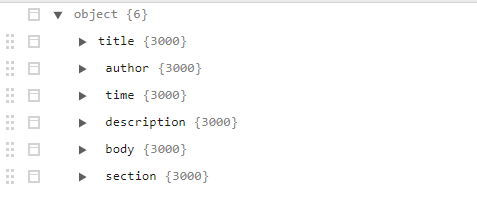
\includegraphics[scale= 0.7]{dataset.png}
\caption{Input dataset in JSON format}
\end{figure}
Each article contains 6 sub-fields:
\begin{description}
\item[-- ]Title: The name of an article
\item[-- ]Author: Author name of an article, could be a person or an organization
\item[-- ]Time: Publishment absolute time to the Internet
\item[-- ]Description: Brief description of the content of an article
\item[-- ]Body: Content in raw text of an article
\item[-- ]Section: Domain of an article 
\end{description}
The dataset can be extended as crawling more data and format into the specified structure.
